\chapter{Evaluations}

\section{Evaluation Metrics}

As NIR colorization has two main application contexts: providing human users more interpretable images and to improve object recognition results by enriching the input with more information.
To assess the effectiveness of both models, we define qualitative evaluation categories and quantitative evaluation metrics based on their ability to achieve these goals.

\subsection{Quantitative Evaluation Metrics}
Due to the unpaired setting, in the quantitative evaluation classic solutions, such as the difference between the absolute intensity values or SSIM \parencite{ssim}, cannot be applied. Fortunately, methods for comparing the general image similarity of two sets, such as FID \parencite{ttur} or
comparing classification results using an off-the-shelf network, are well known to quantitatively assess the quality of image translation.

\subsubsection*{FID}
To measure how close the generated images are to the real images concerning human perception, the \textit{Fréchet Inception Distance} (FID) \parencite{ttur} is a commonly used metric.
It empirically estimates how the human eye perceives images for a set of images and computes the distance between two such set representations.
First, a pre-trained InceptionV3 model evaluates each image of the image set and the activation of the last layer is considered the "human perception approximation".
Then for all activation vectors of the evaluated images in the images set, a multidimensional Gaussian is fitted over those activation vectors.
This is done for two image sets, and later the two Gaussians are compared using the Fréchet distance \parencite{ttur}.
Intuitively, if the generated images are realistic, the statistics of features in a classification network should be similar to the real ones.

\subsubsection*{Evaluation of the FID}
\label{cap:evaluate-fid}

The FID is commonly used on a wide variety of unpaired image comparison tasks.

Conceptually it first, it is only a distance metric between the features of two image sets. 
The features are extracted using 


\subsection{Qualitative Evaluation Methods}
For qualitative evaluation, we define categories on how we determine the superior generated images. These are again based on the two main application contexts.

The first category describes the \textit{naturality} of an image, where the generated images should resemble how humans perceive the world, without artifacts or periodic patterns that can affect visual perception.

The second category refers to the \textit{content preservation} of the input image. This should help humans as well as object detection systems to find and classify animals accurately.

\textit{Hallucinations}, as artifacts or scene elements that are not in the input image, contradict naturality and content preservation, and therefore are undesirable.

\section{Loss-Guided Diffusion and Strongly Guided-Diffusion}
\section{Near-Infrared as Grayscale Approximation}
\section{Diffusion and GAN}
\subsection{Extended Dataset --- Robustness}
\subsection{General Comparison}
Finally, we study the diffusion models performance in comparison to CycleGAN.
An unconditional diffusion model for a resolution of $128 \times 128$ was trained on the RGB domain of the same training dataset as CycleGAN.

First we evaluate the unconditional sampling of the diffusion model and therefore validate \parencite{dif-beat-gan}'s results for image synthesis in still hold for this dataset:

\begin{table}[htp!]
    \centering
    \begin{tabular}{c | c}
        Model                   & FID  $\downarrow$ \\
        \hline\hline
        CycleGAN                & 97.76             \\
        Unconditional Diffusion & 95.73
    \end{tabular}
    \caption{
        \textbf{Quantitative Evaluation.} CycleGAN and the diffusion model trained on Snapshot Serengeti \parencite{serengeti} containing only night NIR and RGB images.
        Comparing the FID calculated between the test dataset and the generated images.
    }
    \label{fig:quantitative-evaluation-unconditional-sampling}
\end{table}

\begin{figure}[htp!]
    \centering
    % TODO choose more animal images
    \setkeys{Gin}{width=1\linewidth}
    \begin{tabularx}{\textwidth}{>{\centering\arraybackslash}X >{\centering\arraybackslash}X >{\centering\arraybackslash}X >{\centering\arraybackslash}X >{\centering\arraybackslash}X >{\centering\arraybackslash}X}
        RGB                                                                                    & CycleGAN                                                                                         & Diffusion                                                                                    & RGB                                                                                    & CycleGAN                                                                                         & Diffusion                                                                                    \\
        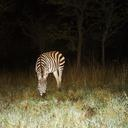
\includegraphics{gfx/unconditional-diffusion-sampling-qual/rgb_S2_B04_R3_IMAG0432.jpg} & \includegraphics{gfx/unconditional-diffusion-sampling-qual/cyclegan_S2_B06_R1_PICT0128_fake.png} & 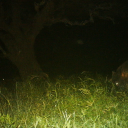
\includegraphics{gfx/unconditional-diffusion-sampling-qual/diffusion_S2_B06_R1_PICT0128.png} & 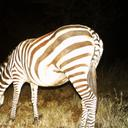
\includegraphics{gfx/unconditional-diffusion-sampling-qual/rgb_S2_B04_R3_IMAG0471.jpg} & \includegraphics{gfx/unconditional-diffusion-sampling-qual/cyclegan_S2_B06_R1_PICT0279_fake.png} & 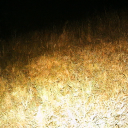
\includegraphics{gfx/unconditional-diffusion-sampling-qual/diffusion_S2_B06_R1_PICT0279.png} \\
        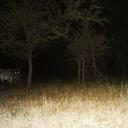
\includegraphics{gfx/unconditional-diffusion-sampling-qual/rgb_S2_B05_R1_IMAG0084.jpg} & \includegraphics{gfx/unconditional-diffusion-sampling-qual/cyclegan_S2_B06_R1_PICT0387_fake.png} & 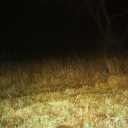
\includegraphics{gfx/unconditional-diffusion-sampling-qual/diffusion_S2_B06_R1_PICT0387.png} & 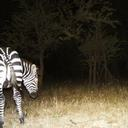
\includegraphics{gfx/unconditional-diffusion-sampling-qual/rgb_S2_B05_R1_IMAG0132.jpg} & \includegraphics{gfx/unconditional-diffusion-sampling-qual/cyclegan_S2_B06_R3_PICT1364_fake.png} & 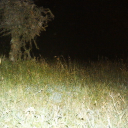
\includegraphics{gfx/unconditional-diffusion-sampling-qual/diffusion_S2_B06_R3_PICT1364.png} \\
        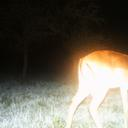
\includegraphics{gfx/unconditional-diffusion-sampling-qual/rgb_S2_B05_R2_IMAG0016.jpg} & \includegraphics{gfx/unconditional-diffusion-sampling-qual/cyclegan_S2_B06_R3_PICT3848_fake.png} & 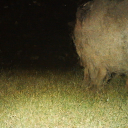
\includegraphics{gfx/unconditional-diffusion-sampling-qual/diffusion_S2_B06_R3_PICT3848.png} & 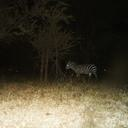
\includegraphics{gfx/unconditional-diffusion-sampling-qual/rgb_S2_B05_R3_IMAG1018.jpg} & \includegraphics{gfx/unconditional-diffusion-sampling-qual/cyclegan_S2_B07_R1_PICT3274_fake.png} & 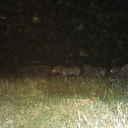
\includegraphics{gfx/unconditional-diffusion-sampling-qual/diffusion_S2_B07_R1_PICT3274.png}
    \end{tabularx}
    \caption{
        \textbf{Qualitative Evaluation.} Left to right: Sample image from the RGB domain of the Serengeti test dataset \parencite{serengeti},
        sample produced by CycleGAN \parencite{mehri2019colorizing} and an unconditional sample produced by the diffusion model \parencite{dif-beat-gan}.
    }
    \label{fig:qualitative-evaluation-unconditional-sampling}
\end{figure}

Qualitatively we observe in \autoref{fig:qualitative-evaluation-unconditional-sampling} that the diffusion model is capable to create realistic images.
The model produced many similar images which do not contain animals, which is not unexpectable since such exist in the training dataset as well.
In cases of animal presence it performances exceptionally well in creating realistic animals with matching lighting.
Only in few cases where trees are generated, branches are not well distinguishing, this is the only flaw which can be observed.

Quantitatively in \autoref{fig:quantitative-evaluation-unconditional-sampling} we see, the diffusion network only slightly outperforms CycleGAN's performance.
This may be caused by the usage of a smaller U-Net generator, less training iterations and a smaller dataset compared to \parencite{dif-beat-gan} which are all trade-off which
had to be made due to a lack of ultra-high performant computational resources.
Nevertheless, it can be argued that this unconditional diffusion model is capable enough to be a basis for a good colorization.


\begin{table}[htp!]
    \centering
    \begin{tabular}{c | c}
        Model                 & FID  $\downarrow$ \\
        \hline\hline
        CycleGAN              & 98.10             \\
        Conditional Diffusion & 103.71
    \end{tabular}
    \caption{
        \textbf{Quantitative Evaluation.} CycleGAN and the diffusion model trained on Snapshot Serengeti \parencite{serengeti} containing only night NIR and RGB images.
        Comparing the FID calculated between the test dataset and the generated images.
    }
    \label{fig:quantitative-evaluation-conditiona-sampling}
\end{table}

\begin{figure}
    \centering
    \setkeys{Gin}{width=1\linewidth}
    \begin{tabularx}{\textwidth}{>{\centering\arraybackslash}X >{\centering\arraybackslash}X >{\centering\arraybackslash}X >{\centering\arraybackslash}X >{\centering\arraybackslash}X >{\centering\arraybackslash}X}
        NIR                                                                                  & CycleGAN                                                                                       & Diffusion                                                                                  & NIR                                                                                  & CycleGAN                                                                                       & Diffusion                                                                                  \\
        \includegraphics{gfx/conditional-diffusion-sampling-qual/nir_S2_B06_R1_PICT0128.jpg} & \includegraphics{gfx/conditional-diffusion-sampling-qual/cyclegan_S2_B06_R1_PICT0128_fake.png} & 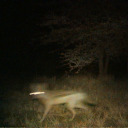
\includegraphics{gfx/conditional-diffusion-sampling-qual/diffusion_S2_B06_R1_PICT0128.png} & \includegraphics{gfx/conditional-diffusion-sampling-qual/nir_S2_B06_R1_PICT0279.jpg} & \includegraphics{gfx/conditional-diffusion-sampling-qual/cyclegan_S2_B06_R1_PICT0279_fake.png} & 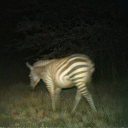
\includegraphics{gfx/conditional-diffusion-sampling-qual/diffusion_S2_B06_R1_PICT0279.png} \\
        \includegraphics{gfx/conditional-diffusion-sampling-qual/nir_S2_B06_R1_PICT0387.jpg} & \includegraphics{gfx/conditional-diffusion-sampling-qual/cyclegan_S2_B06_R1_PICT0387_fake.png} & 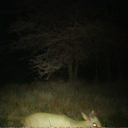
\includegraphics{gfx/conditional-diffusion-sampling-qual/diffusion_S2_B06_R1_PICT0387.png} & \includegraphics{gfx/conditional-diffusion-sampling-qual/nir_S2_B06_R3_PICT1364.jpg} & \includegraphics{gfx/conditional-diffusion-sampling-qual/cyclegan_S2_B06_R3_PICT1364_fake.png} & 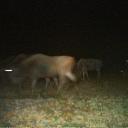
\includegraphics{gfx/conditional-diffusion-sampling-qual/diffusion_S2_B06_R3_PICT1364.png} \\
        \includegraphics{gfx/conditional-diffusion-sampling-qual/nir_S2_B06_R3_PICT3848.jpg} & \includegraphics{gfx/conditional-diffusion-sampling-qual/cyclegan_S2_B06_R3_PICT3848_fake.png} & 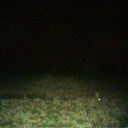
\includegraphics{gfx/conditional-diffusion-sampling-qual/diffusion_S2_B06_R3_PICT3848.png} & 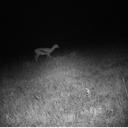
\includegraphics{gfx/conditional-diffusion-sampling-qual/nir_S2_B07_R1_PICT3274.jpg} & \includegraphics{gfx/conditional-diffusion-sampling-qual/cyclegan_S2_B07_R1_PICT3274_fake.png} & 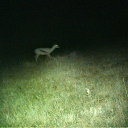
\includegraphics{gfx/conditional-diffusion-sampling-qual/diffusion_S2_B07_R1_PICT3274.png}
    \end{tabularx}
    \caption{
        \textbf{Qualitative Evaluation.} Left to right: Image from the NIR domain of the Serengeti test dataset \parencite{serengeti},
        corresponding image generated by CycleGAN \parencite{mehri2019colorizing} and corresponding sample generated by our diffusion model approach.
    }
    \label{fig:qualitative-evaluation-conditional-sampling}
\end{figure}


We compare performances of our trained CycleGAN with our conditional diffusion network.
In this case strong guidance with the NIR $\approx$ Intensity approximation is used.
\autoref{fig:quantitative-evaluation-conditiona-sampling} indicates strong performance of the conditional
diffusion network only, $\sim 6$ FID points worse than CycleGAN.
Considering the flaws analyzed and observed in \autoref{cap:evaluate-fid} those points are only a small difference.
Furthermore, qualitatively we can also observe those generated images are faithful to the input image (\autoref{fig:qualitative-evaluation-conditional-sampling}).
It is to be mentioned that faithfulness to the input image is not a quality learned by the network, but a design choice of the sampling procedure.
Additionally, colors estimated by the diffusion model appear reasonable.
Weaknesses in the colorization are observable when analyzing the zebra image:
While CycleGAN colorizes the main zebra body as black and white, the diffusion network produces an orange-black zebra.
This can be traced back to a conceptional weakness.
The diffusion network is forced to reuse the intensity of the NIR image.
The zebra in the NIR image is gray-black and therefore the network is not capable in generating high intensity pixels.
CycleGAN on the other-hand is not restricted by design to change the intensity.
It is merely trained to produce invertible images.


We analyze this concrete weakness of this sampling technique for colorization further.
First we analyze the intensity generated by the CycleGAN.
In \autoref{fig:heatmap-cycle-gan-intensity}, we first observe the pattern,
that CycleGAN does especially enlighten the foreground and with that the lower regions of the image.
The same holds for animals in the foreground such as the fox or zebra.

A solid explanation for this behavior can be found while manually comparing the intensity of colored images and the near
infrared images from night in the Serengeti dataset \parencite{serengeti}:
Generally the light in RGB images appears to be stronger and therefore foreground objects are better illuminated.
By forcing the intensity of the NIR image on the diffusion model such distinct features of the incandescent images is not achievable.

\begin{figure}[htp!]
    \centering
    % TODO Better integration (using pdf or so); Best: Direct latex code 
    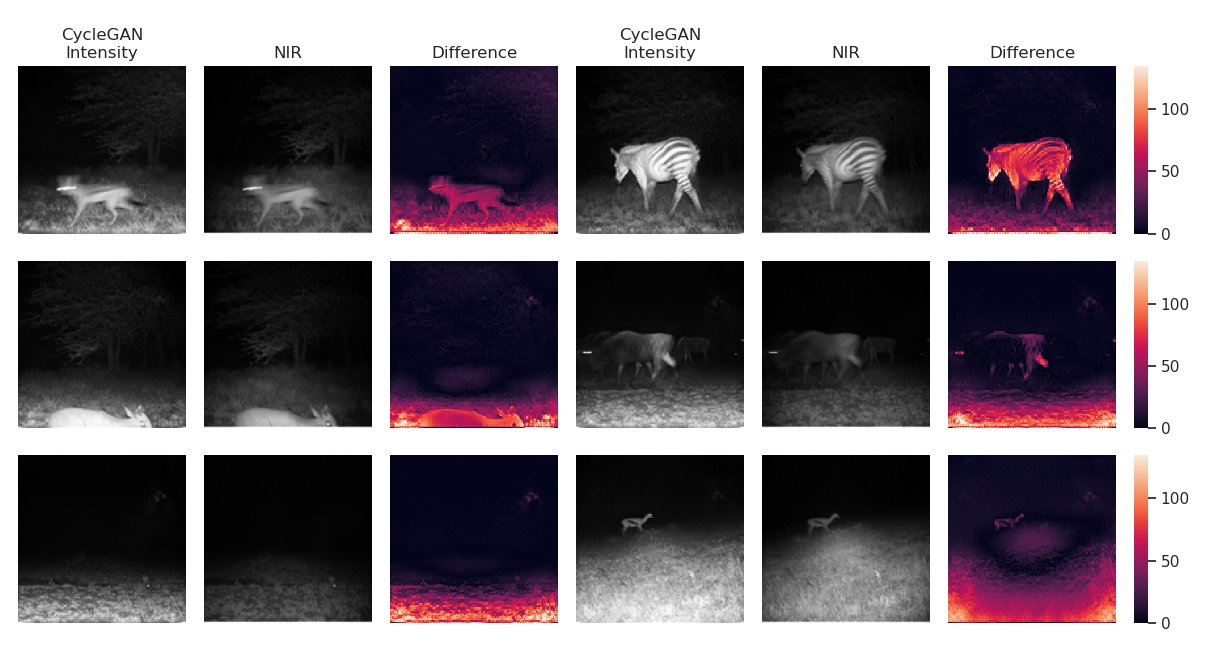
\includegraphics[width=\textwidth]{gfx/heatmap-nir-cycle-gan-intensity-diff.png}
    \caption{
        Absolute difference between CycleGAN's intensity and the NIR image.
        Left to Right: Intensity calculated by images generated by CycleGAN, Near-Infared image \parencite{serengeti} and difference between both.
    }
    \label{fig:heatmap-cycle-gan-intensity}
\end{figure}

We hypothesize that the fixed intensity is the main weakness of our approach.
To validate our hypothesis, we use the intensities of the CycleGAN model as conditioning input for our diffusion model instead of the near-infrared values.

\begin{figure}[htp!]
    \centering
    \setkeys{Gin}{width=1\linewidth}
    \begin{tabularx}{\textwidth}{>{\centering\arraybackslash}X >{\centering\arraybackslash}X >{\centering\arraybackslash}X >{\centering\arraybackslash}X >{\centering\arraybackslash}X >{\centering\arraybackslash}X}
        NIR                                                                              & CycleGAN                                                                                   & Diffusion with CycleGAN Input                                                                    & NIR                                                                              & CycleGAN                                                                                   & Diffusion with CycleGAN Input                                                                    \\
        \includegraphics{gfx/conditional-with-cycle-gan-qual/nir_S2_B06_R1_PICT0128.jpg} & \includegraphics{gfx/conditional-with-cycle-gan-qual/cyclegan_S2_B06_R1_PICT0128_fake.png} & 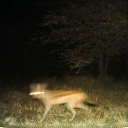
\includegraphics{gfx/conditional-with-cycle-gan-qual/diff_cycle_gan_S2_B06_R1_PICT0128_fake.png} & \includegraphics{gfx/conditional-with-cycle-gan-qual/nir_S2_B06_R1_PICT0279.jpg} & 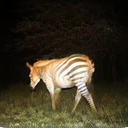
\includegraphics{gfx/conditional-with-cycle-gan-qual/cyclegan_S2_B06_R1_PICT0279_fake.png} & 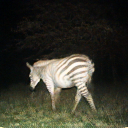
\includegraphics{gfx/conditional-with-cycle-gan-qual/diff_cycle_gan_S2_B06_R1_PICT0279_fake.png} \\
        \includegraphics{gfx/conditional-with-cycle-gan-qual/nir_S2_B06_R1_PICT0387.jpg} & \includegraphics{gfx/conditional-with-cycle-gan-qual/cyclegan_S2_B06_R1_PICT0387_fake.png} & 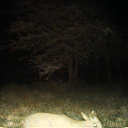
\includegraphics{gfx/conditional-with-cycle-gan-qual/diff_cycle_gan_S2_B06_R1_PICT0387_fake.png} & \includegraphics{gfx/conditional-with-cycle-gan-qual/nir_S2_B06_R3_PICT1364.jpg} & \includegraphics{gfx/conditional-with-cycle-gan-qual/cyclegan_S2_B06_R3_PICT1364_fake.png} & 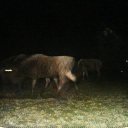
\includegraphics{gfx/conditional-with-cycle-gan-qual/diff_cycle_gan_S2_B06_R3_PICT1364_fake.png} \\
        \includegraphics{gfx/conditional-with-cycle-gan-qual/nir_S2_B06_R3_PICT3848.jpg} & \includegraphics{gfx/conditional-with-cycle-gan-qual/cyclegan_S2_B06_R3_PICT3848_fake.png} & \includegraphics{gfx/conditional-with-cycle-gan-qual/diff_cycle_gan_S2_B06_R3_PICT3848_fake.png} & \includegraphics{gfx/conditional-with-cycle-gan-qual/nir_S2_B07_R1_PICT3274.jpg} & \includegraphics{gfx/conditional-with-cycle-gan-qual/cyclegan_S2_B07_R1_PICT3274_fake.png} & \includegraphics{gfx/conditional-with-cycle-gan-qual/diff_cycle_gan_S2_B07_R1_PICT3274_fake.png}
    \end{tabularx}
    \caption{
        % TODO
        Absolute difference between CycleGAN's intensity and the NIR image.
        Left to Right: Intensity calculated by images generated by CycleGAN, Near-Infared image \parencite{serengeti} and difference between both.
    }
    \label{fig:qualitative-evaluation-cyclegan-conditional-sampling}
\end{figure}

In \autoref{fig:qualitative-evaluation-cyclegan-conditional-sampling} we see that not only is the diffusion model more than capable in colorizing these pictures,
it also exceeds CycleGAN's color choices. While the zebra of CycleGAN has an orange outline at the head where it should not, the diffusion model does not make this mistake
which results in overall more realistic images.

This subtle difference between the CycleGAN and the diffusion model samples with CycleGAN intensity inputs is also visible while comparing the images quantitatively in \autoref{fig:quantitative-evaluation-cyclegan-conditional-sampling}.
The diffusion model performs better than CycleGAN when the intensities are appropriate.
It is not expected by the diffusion model to perform better than in the unconditional setting (assuming test dataset and train dataset are divided appropriately). 
Because the diffusion model in the unconditional setting only performs $1.2$ FID points better (\autoref{fig:quantitative-evaluation-unconditional-sampling}) it is reasonable that those samples are the best this diffusion model can produce.
This proves that the main weakness of our approach lies in the fixed intensity. 

\begin{table}[htp!]
    \centering
    \begin{tabular}{c | c}
        Model                                    & FID  $\downarrow$  \\
        \hline\hline
        CycleGAN                                 & 98.10              \\
        Diffusion with CycleGAN Intensity Inputs & \textbf{97.21} \\
        Diffusion with NIR Inputs                & 104.04
    \end{tabular}
    \caption{
        % TODO
        \textbf{Quantitative Evaluation.} CycleGAN and the diffusion model trained on Snapshot Serengeti \parencite{serengeti} containing only night NIR and RGB images.
        Comparing the FID calculated between the test dataset and the generated images.
    }
    \label{fig:quantitative-evaluation-cyclegan-conditional-sampling}
\end{table}